\section{Gekoppelte LC-Schwingkreise}


\subsection{Versuchsbeschreibung}

In diesem Versuch werden zwei Schwingkreise induktiv miteinander gekoppelt. Speziell werden hier die beiden Fundamentalschwingungen bei gleichsinniger und gegensinniger Anregung und eine Schwebung aufgezeichnet.

\begin{figure}[H]
\centering
\begin{tikzpicture}
% Linke Schwingkreise
\draw (0,0.2) -- (-1,0.2) to [rmeterwa, t=$U_1$] (-1,1.8) -- (0,1.8);
\draw (0.8,0) node[ocirc]{} -- (0,0) to [C, a=$C$] (0,2) -- (2,2) to [cute inductor, a=$L$] (2,0) -- (1.2,0) node[ocirc]{};
\draw (3.55,0) node[ocirc]{} -- (2.75,0) to [cute inductor, a=$L$] (2.75,2) -- (4.75,2) to[C, a=$C$] (4.75,0) -- (3.95,0) node[ocirc]{};
\draw (4.75,0.2) -- (5.75,0.2) to [rmeterwa, t=$U_2$] (5.75,1.8) -- (4.75,1.8);
\draw (2,0) to [normal open switch] (2,-1) -- (0,-1) -- (0,0);
\draw (2.75,0) to [normal open switch] (2.75,-1) -- (4.75,-1) -- (4.75,0);
\draw[dashed, thin] (2.15,-0.5) -- (2.85,-0.5); 


% Rechte Schwingkreise
\draw (8,0.2) -- (7,0.2) to [rmeterwa, t=$U_1$] (7,1.8) -- (8,1.8);
\draw (8.8,0) node[ocirc]{} -- (8,0) to [C, a=$C$] (8,2) -- (10,2) to [cute inductor, a=$L$] (10,0) -- (9.2,0) node[ocirc]{};
\draw (11.55,0) node[ocirc]{} -- (10.75,0) to [cute inductor, a=$L$] (10.75,2) -- (12.75,2) to[C, a=$C$] (12.75,0) -- (11.95,0) node[ocirc]{};
\draw (12.75,0.2) -- (13.75,0.2) to [rmeterwa, t=$U_2$] (13.75,1.8) -- (12.75,1.8);
\draw (10,0) to [normal open switch] (10,-1) -- (8,-1) -- (8,0);
\draw (10.75,0) to [normal open switch] (10.75,-1) -- (12.75,-1) -- (12.75,0);
\draw[dashed, thin] (10.15,-0.5) -- (10.85,-0.5); 

\end{tikzpicture}
\caption{Fundamentalschwingungen der gekoppelten Schwingkreise bei gleichsinniger (links) und gegensinniger Anregung (rechts)}
\end{figure}

Bei überbrückter Spannungsquelle gelten für den gekoppelten Schwingkreis die folgenden Differentialgleichungen 
\begin{align*}
\ddot I_1 + k \ddot I_2 + \frac{1}{LC}I_1 &= 0 \\
\ddot I_2 + k \ddot I_1 + \frac{1}{LC}I_2 &= 0
\end{align*}
Dabei bezeichnet $k \in (0,1)$ die Kopplung der beiden Schwingkreise. 
Mit den sogenannten \textit{Fundamentalströmen} $I_+ = I_1 + I_2$ und $I_- = I_1 - I_2$ erhält man durch Addition bzw. Subtraktion der obigen Gleichungen und anschließendem Umformen
\begin{align*}
\ddot I_+ + \frac{1}{LC(1+k)} I_+ = 0 \\
\ddot I_- + \frac{1}{LC(1-k)} I_- = 0
\end{align*}
Daraus ergeben sich harmonische Schwingungen mit den Kreisfrequenzen 
$$\omega_+ = \frac{\omega_0}{\sqrt{1+k}} \hspace{0.2cm} \text{ und } \hspace{0.2cm} \omega_- = \frac{\omega_0}{\sqrt{1+k}}.$$
Dabei ist $\omega_0 = \frac{1}{\sqrt{LC}}$ die Kreisfrequenz der ungekoppelten Schwingung. Mithilfe der Fundamentalschwingungen lässt sich dann der Kopplungsgrad bestimmen
$$k = \frac{f_-^2 - f_+^2}{f_-^2 + f_+^2}.$$
Bei Messung einer Schwebung mit Schwebungsfrequenz $f_s$ und Frequenz der gekoppelten Schwingung $f_k$ kann man die Fundamentalschwingungen gemäß
$$f_k = \frac{f_- + f_+}{2} \hspace{0.2cm} \text{ und } \hspace{0.2cm} f_s = \frac{f_- - f_+}{2}$$
bestimmen. Aufgrund der unvermeidbaren Dämpfung der beiden Schwingkreise sind die Extrema des einen Schwingkreises gegen die Nulldurchgänge des anderen verschoben. Für Kopplungen $k < 0.2$ gilt näherungsweise für die zeitliche Verschiebung

\begin{equation}\label{eq:delta_t}
\Delta t \approx \frac{1}{\omega_s} \left( \frac{\pi}{2} - \arctan\left(  \frac kR \sqrt{\frac LC}\right) \right)
\end{equation}



\subsection{Schwebung}


\subsubsection{Versuchsaufbau}

\begin{figure}[H]
\centering
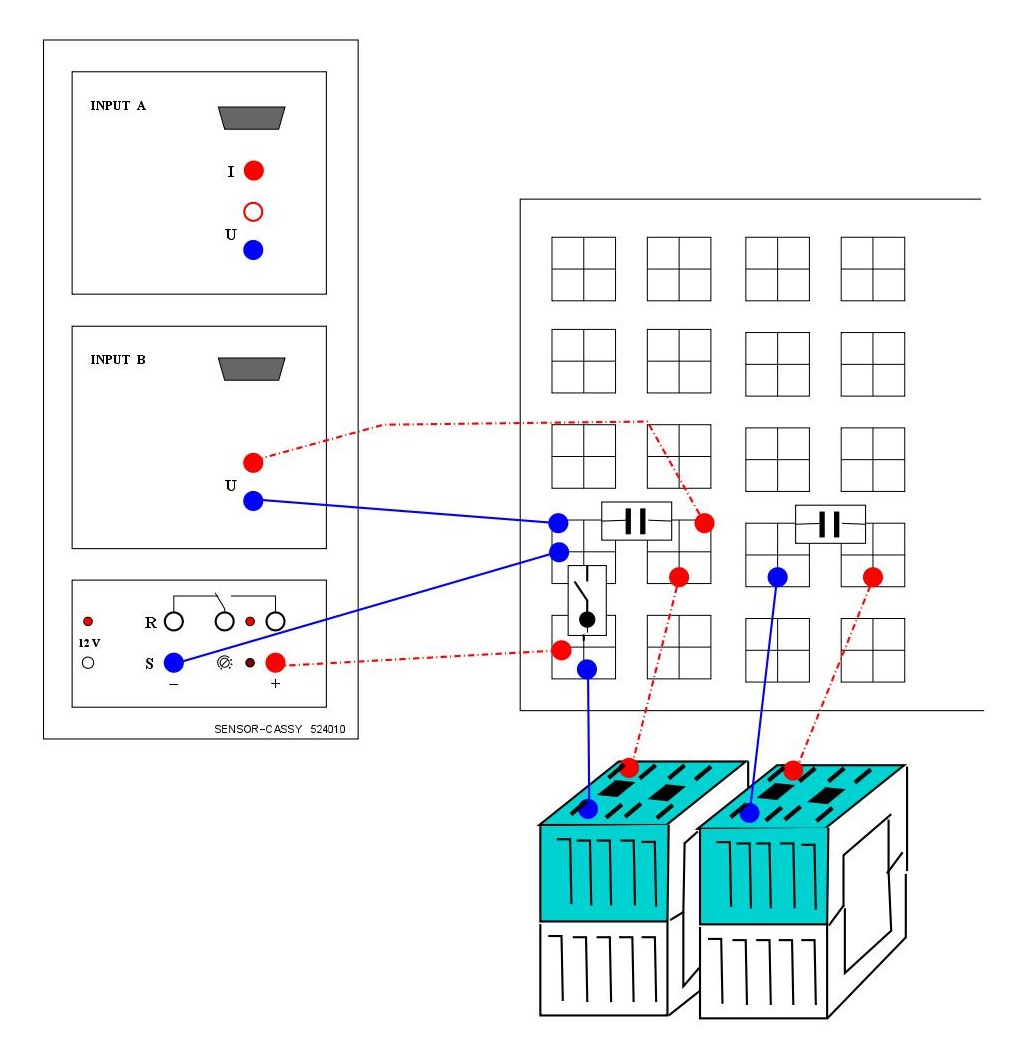
\includegraphics[width=0.6\textwidth]{bilder/aufbau_schwebung.jpg}
\caption{Aufbau zur Erzeugung einer Schwebung}
\label{abb:aufbau_schweb}
\end{figure}

Zur Erzeugung einer Schwebung wird nur einer der beiden Schwingkreise angeregt. Die Schwingkreise werden gemäß Abbildung \ref{abb:aufbau_schweb} auf der Rastersteckplatte aufgebaut. Als Schalter dient dabei ein Taster. Im ersten Schwingkreis werden Kondensator und Spule aus dem ersten Versuch verwendet. Für den zweiten Schwingkreis werden baugleiche Teile benutzt.


\subsubsection{Versuchsdurchführung}

Kondensator 1 wird mit $U_0 = 9.5 \, \mathrm V$ aufgeladen. Die Spannung am ersten Kondensator $U_1$ wird im Eingang A des ersten Sensor-CASSYs und die Spannung am zweiten Kondensator $U_2$ wird im Eingang A des zweiten Sensor-CASSYs gemessen. Für die Messungen werden folgende Messparameter verwendet:

\begin{enumerate}[-]
\setlength{\itemsep}{-5pt} 
\item Messart: automatische Aufnahme
\item Messbereich: $\pm$10 V
\item Messintervall: $10\,\mu$s 
\item Messungen: $8000$
\item Messzeit: $80\,$ms
\end{enumerate}

Die Messung wird dabei durch einen Trigger auf die fallende Flanke von $U_1$ bei 6.7 V gestartet. Es werden Schwebungen in drei verschiedenen Konfigurationen aufgezeichnet. Bei Schwebung 1 befinden sich die Spulen direkt aneinander. Bei Schwebung 2 haben die Spulen einen Abstand von etwa 5 cm und bei Schwebung 3 werden die Spulen direkt aneinander auf einen Eiskern gepackt. Bei einer Messung mit einer LCR-Messbrücke von Telemeter Electronic ergaben sich für die Bauteile die folgenden Werte:

\begin{table}[H]
\centering
\begin{tabular}{c|c|c}
Schwingkreis & Kapazität / nF & Induktivität / mH\\
\hline
1 & $984.2 \pm 0.2$ & $9.03 \pm 0.01$ \\
2 & $980.1 \pm 0.1$ & $9.00 \pm 0.01$
\end{tabular}
\end{table} 

Die Fehler wurden dabei anhand der Fluktuation des angezeigten Wertes geschätzt.

\subsubsection{Versuchsauswertung}

Die Rohdaten zu Schwebung 1 sind in Abbildung \ref{abb:schwebung_roh} beispielhaft zu sehen.

\begin{figure}[H]
\centering
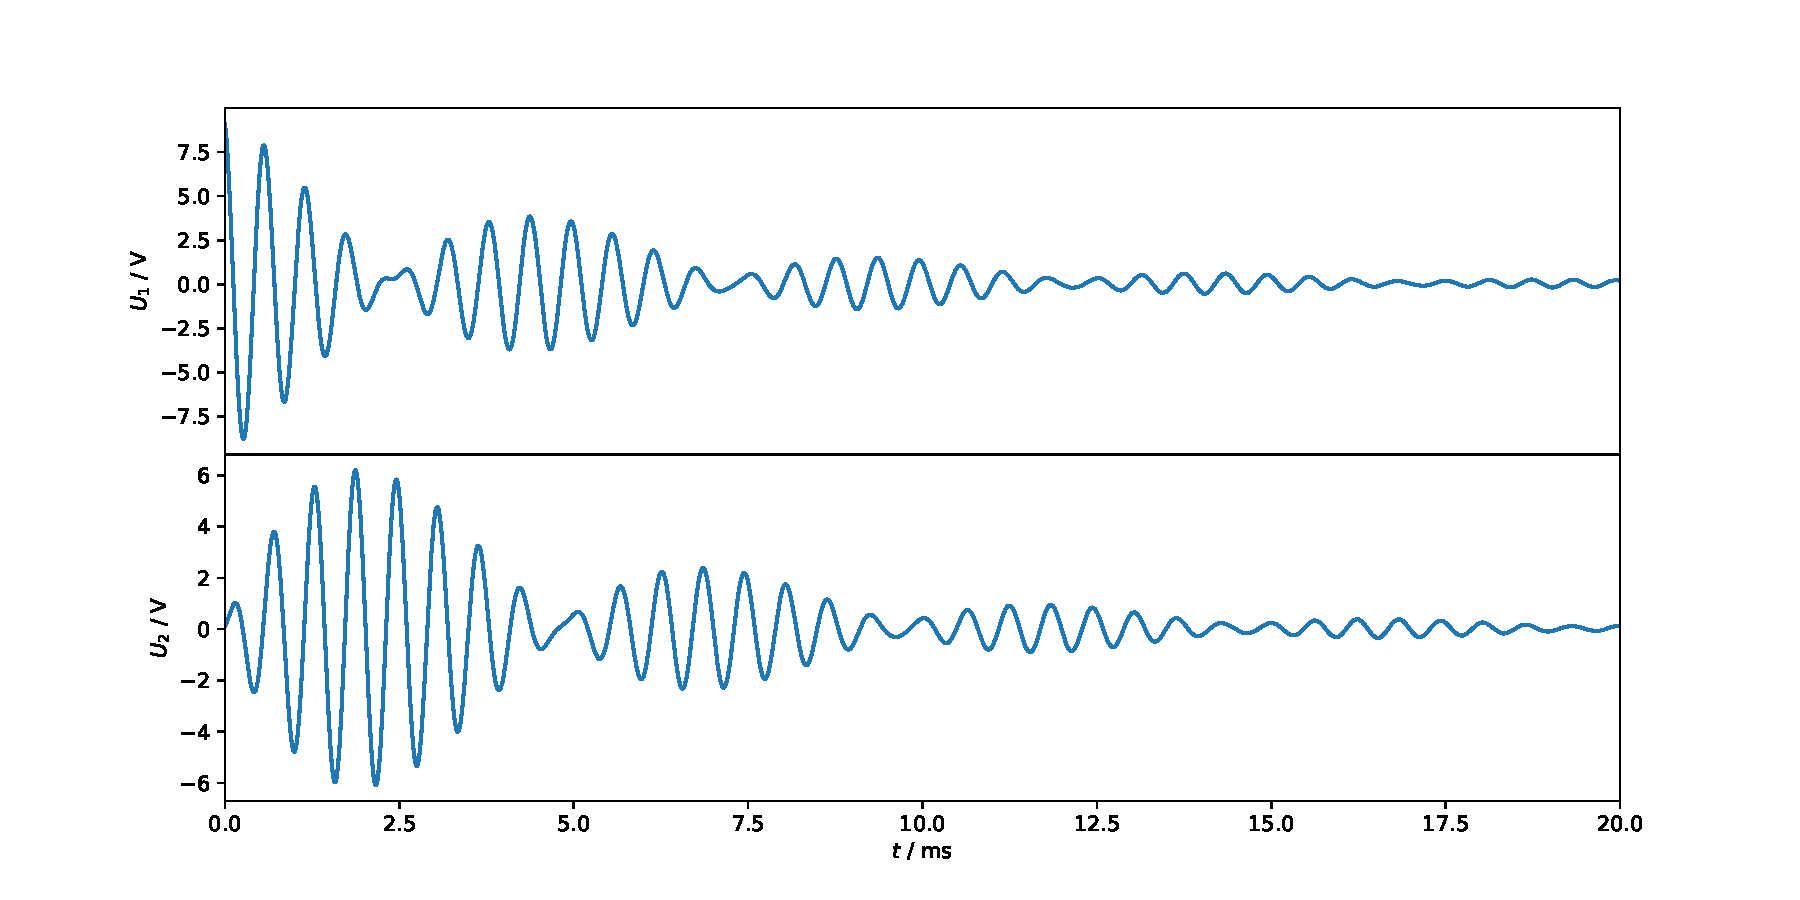
\includegraphics[width=\textwidth]{plots/schwebung_roh.pdf}
\caption{Rohdaten der Schwebung}
\label{abb:schwebung_roh}
\end{figure}

Da sich die Periodendauer der Schwebung bei den beiden anderen Schwebungen garnicht anhand der Schwebungsmaxima bestimmen lässt, wird ausschließlich eine Auswertung mittels FFT vorgenommen. Die Frequenzspektren für alle drei Konfigurationen sind in Abbildung \ref{abb:FFT_schwebung} zu sehen. Diese wurden aus der Spannung am ersten Kondensator berechnet.

\begin{figure}
\centering
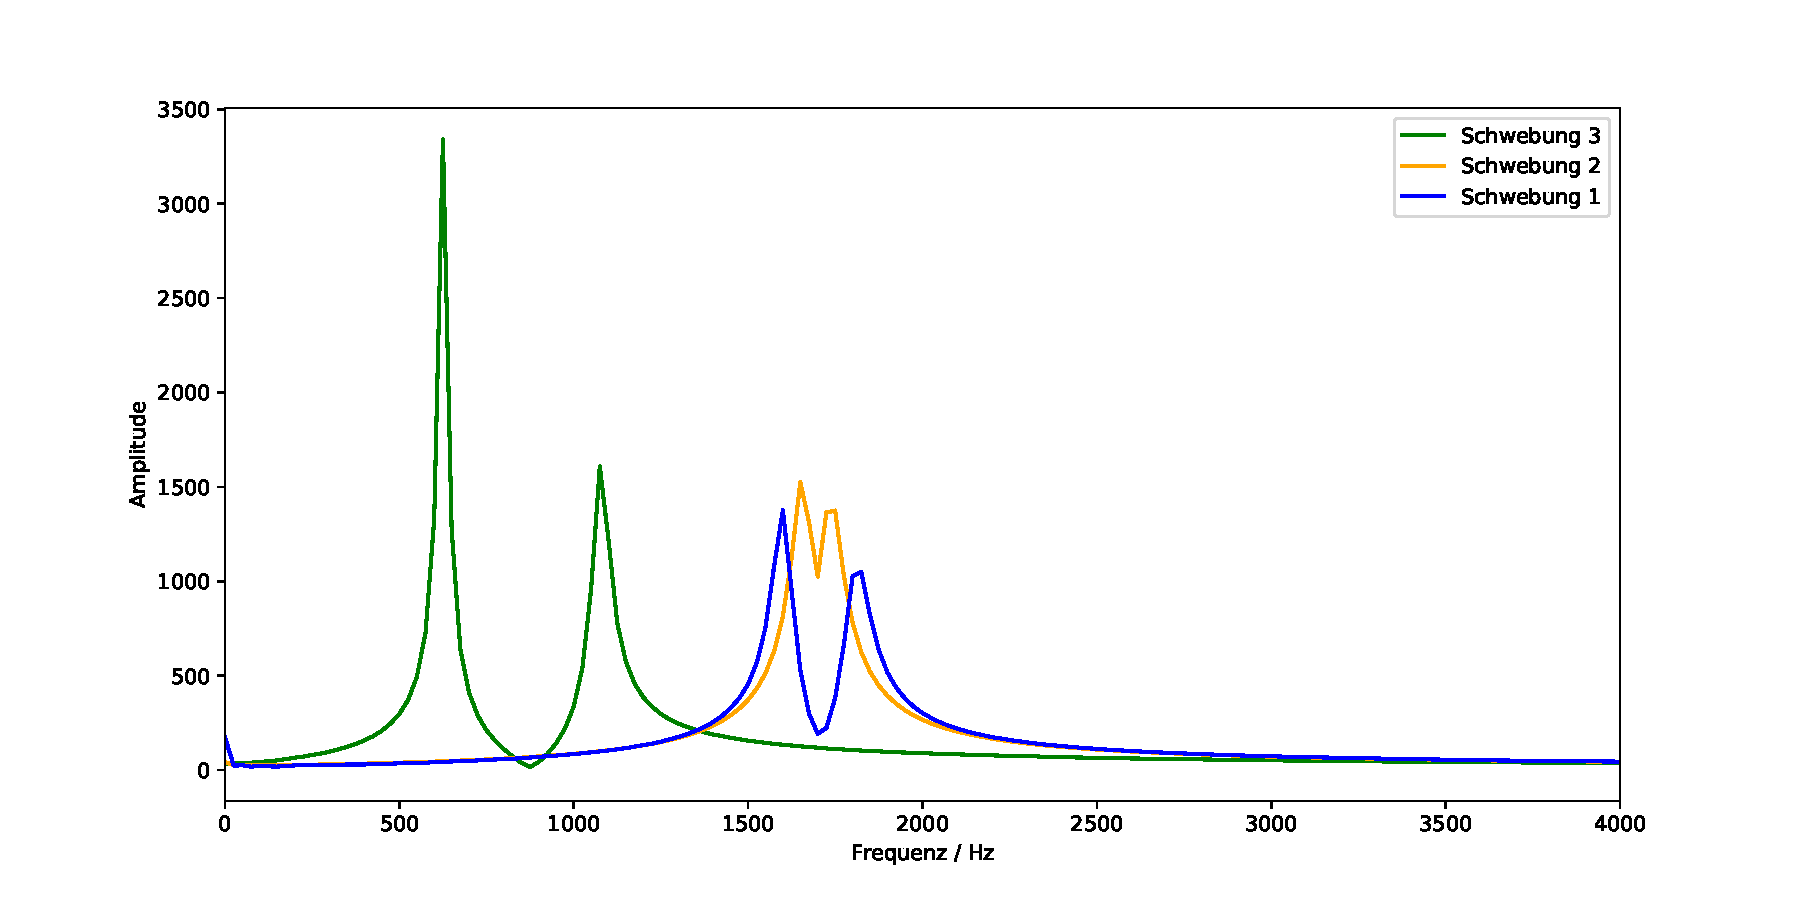
\includegraphics[width=\textwidth]{plots/FFT_schwebungen.pdf}
\caption{Frequenzspektren der drei Schwebungen}
\label{abb:FFT_schwebung}
\end{figure}

Man erkennt gut, dass mit zunehmender Dämpfung die Peaks weiter auseinander liegen und der Mittelwert der Peaks sich zu kleineren Frequenzen verschiebt. Mit der Peak-Schwerpunktmethode ergeben sich die Frequenzen in Tabelle \ref{tab:freq_schweb}. Als Fehler wird dabei die Frequenzdifferenz zwischen Argument-Maximum und Peakschwerpunkt verwendet.

\begin{table}[H]
\centering
\begin{tabular}{c|c|c}
Schwebung & $f_+$ / Hz & $f_-$ / Hz \\
\hline
1 & $1598.65 \pm 0.95$ & $1832.1 \pm 7.5$ \\
2 & $1639 \pm 11$ & $1727 \pm 23$ \\
3 & $631.8 \pm 6.9$ & $1094 \pm 19$
\end{tabular}
\caption{Frequenzen aus FFT}
\label{tab:freq_schweb}
\end{table}

Die Spannung am zweiten Kondensator liefert hier identische Werte. Mithilfe der Frequenzen lassen sich nun die Kopplungsgrade der drei Konfigurationen berechnen. Es gilt
$$k = \frac{f_-^2 - f_+^2}{f_-^2 + f_+^2}.$$
Mittels Gaußscher Fehlerfortpflanzung lässt sich der Fehler auf $k$ zu
$$\sigma_k = \frac{4f_-f_+}{(f_-^2+f_+^2)^2} \sqrt{f_+^2 \sigma_{f_-}^2 + f_-^2 \sigma_{f_+}^2}$$
bestimmen. Es ergeben sich die Werte in Tabelle \ref{tab:kopplung}.

\begin{table}[H]
\centering
\begin{tabular}{c|c}
Schwebung & $k$ \\
\hline
1 & $0.1355 \pm 0.0041$ \\
2 & $0.0522 \pm 0.0146$ \\
3 & $0.4999 \pm 0.0155$
\end{tabular}
\caption{Berechnete Kopplungsgrade}
\label{tab:kopplung}
\end{table}

Wir wollen nun noch überprüfen, ob die erwartete Zeitverschiebung aus Gleichung \ref{eq:delta_t} zutrifft. Die Beziehung gilt dabei nur für die Schwebungen 1 und 2. Da sich bei Schwebung 2 die Verschiebung nicht ablesen lässt, werten wir ausschließlich Schwebung 1 aus. Es lassen sich hier zwei Maxima/Nulldurchgänge auswerten. Abbildung \ref{abb:delta_t_bsp} veranschaulicht das Ablesen der Zeitpunkte und den Ablesefehler. 

\begin{figure}[H]
\centering
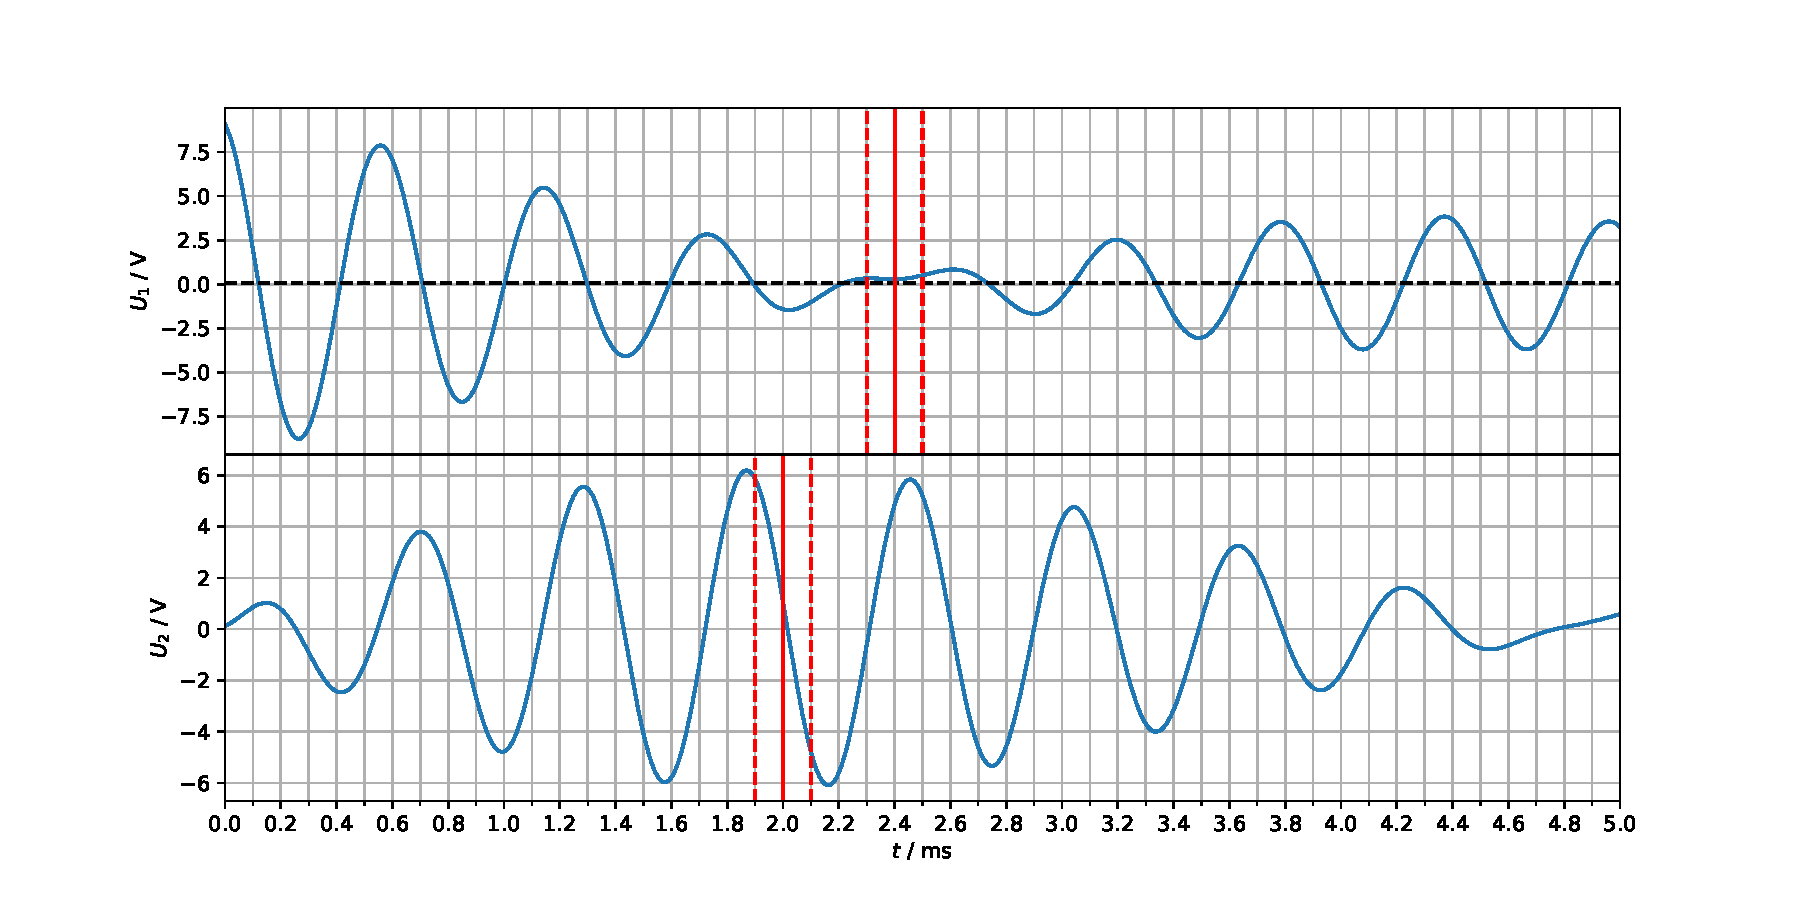
\includegraphics[width=\textwidth]{plots/delta_t_bsp.pdf}
\caption{Bestimmung der Nulldurchgänge/Maxima}
\label{abb:delta_t_bsp}
\end{figure}

Die abgelesenen Zeitpunkte sind in Tabelle \ref{tab:delta_t_zeiten} aufgeführt.

\begin{table}[H]
\centering
\begin{tabular}{c|c|c}
& $t_1$ / ms & $t_2$ / ms \\
\hline
Nulldurchgang $U_1$ & $2.4 \pm 0.1$ & $7.3 \pm 0.1$ \\
Maximum $U_2$ & $2.0 \pm 0.1$ & $6.9 \pm 0.1$
\end{tabular}
\caption{Abgelesene Zeitpunkte der Nulldurchgänge/Maxima}
\label{tab:delta_t_zeiten}
\end{table}

Nach Differenzbildung und gewichteter Mittelung ergibt sich mit dem inneren Fehler $\Delta t = (0.4 \pm 0.1) \, \mathrm{ms}$. Zum Vergleich berechnen wir die erwartete Zeitverschiebung
$$\Delta t_e \approx 0.495 \, \mathrm{ms}.$$
Dabei wurde für den Widerstand der Wert des Restwiderstandes aus dem ersten Versuch verwendet. Die abgelesene Verschiebung stimmt also innerhalb der Unsicherheiten mit der Erwartung überein.

\subsubsection{Fazit}

In diesem Versuch konnten einige qualitative Aussagen bestätigt werden. Zum einen konnte man sehen, dass die Peaks im Frequenzspektrum mit zunehmender Dämpfung zu kleineren Frequenzen verschoben sind und weiter auseinander liegen. Zudem konnte auch die erwartete Zeitverschiebung zwischen den Nulldurchgängen des einen und den Extrema des anderen Schwingkreises bestätigt werden. Nebenbei wurden die Kopplungsgrade $k$ für die erste und dritte Schwebung auf etwa 3 \% genau bestimmt.



\subsection{Fundamentalschwingungen}


\subsubsection{Versuchsaufbau}

\begin{figure}[H]
\centering
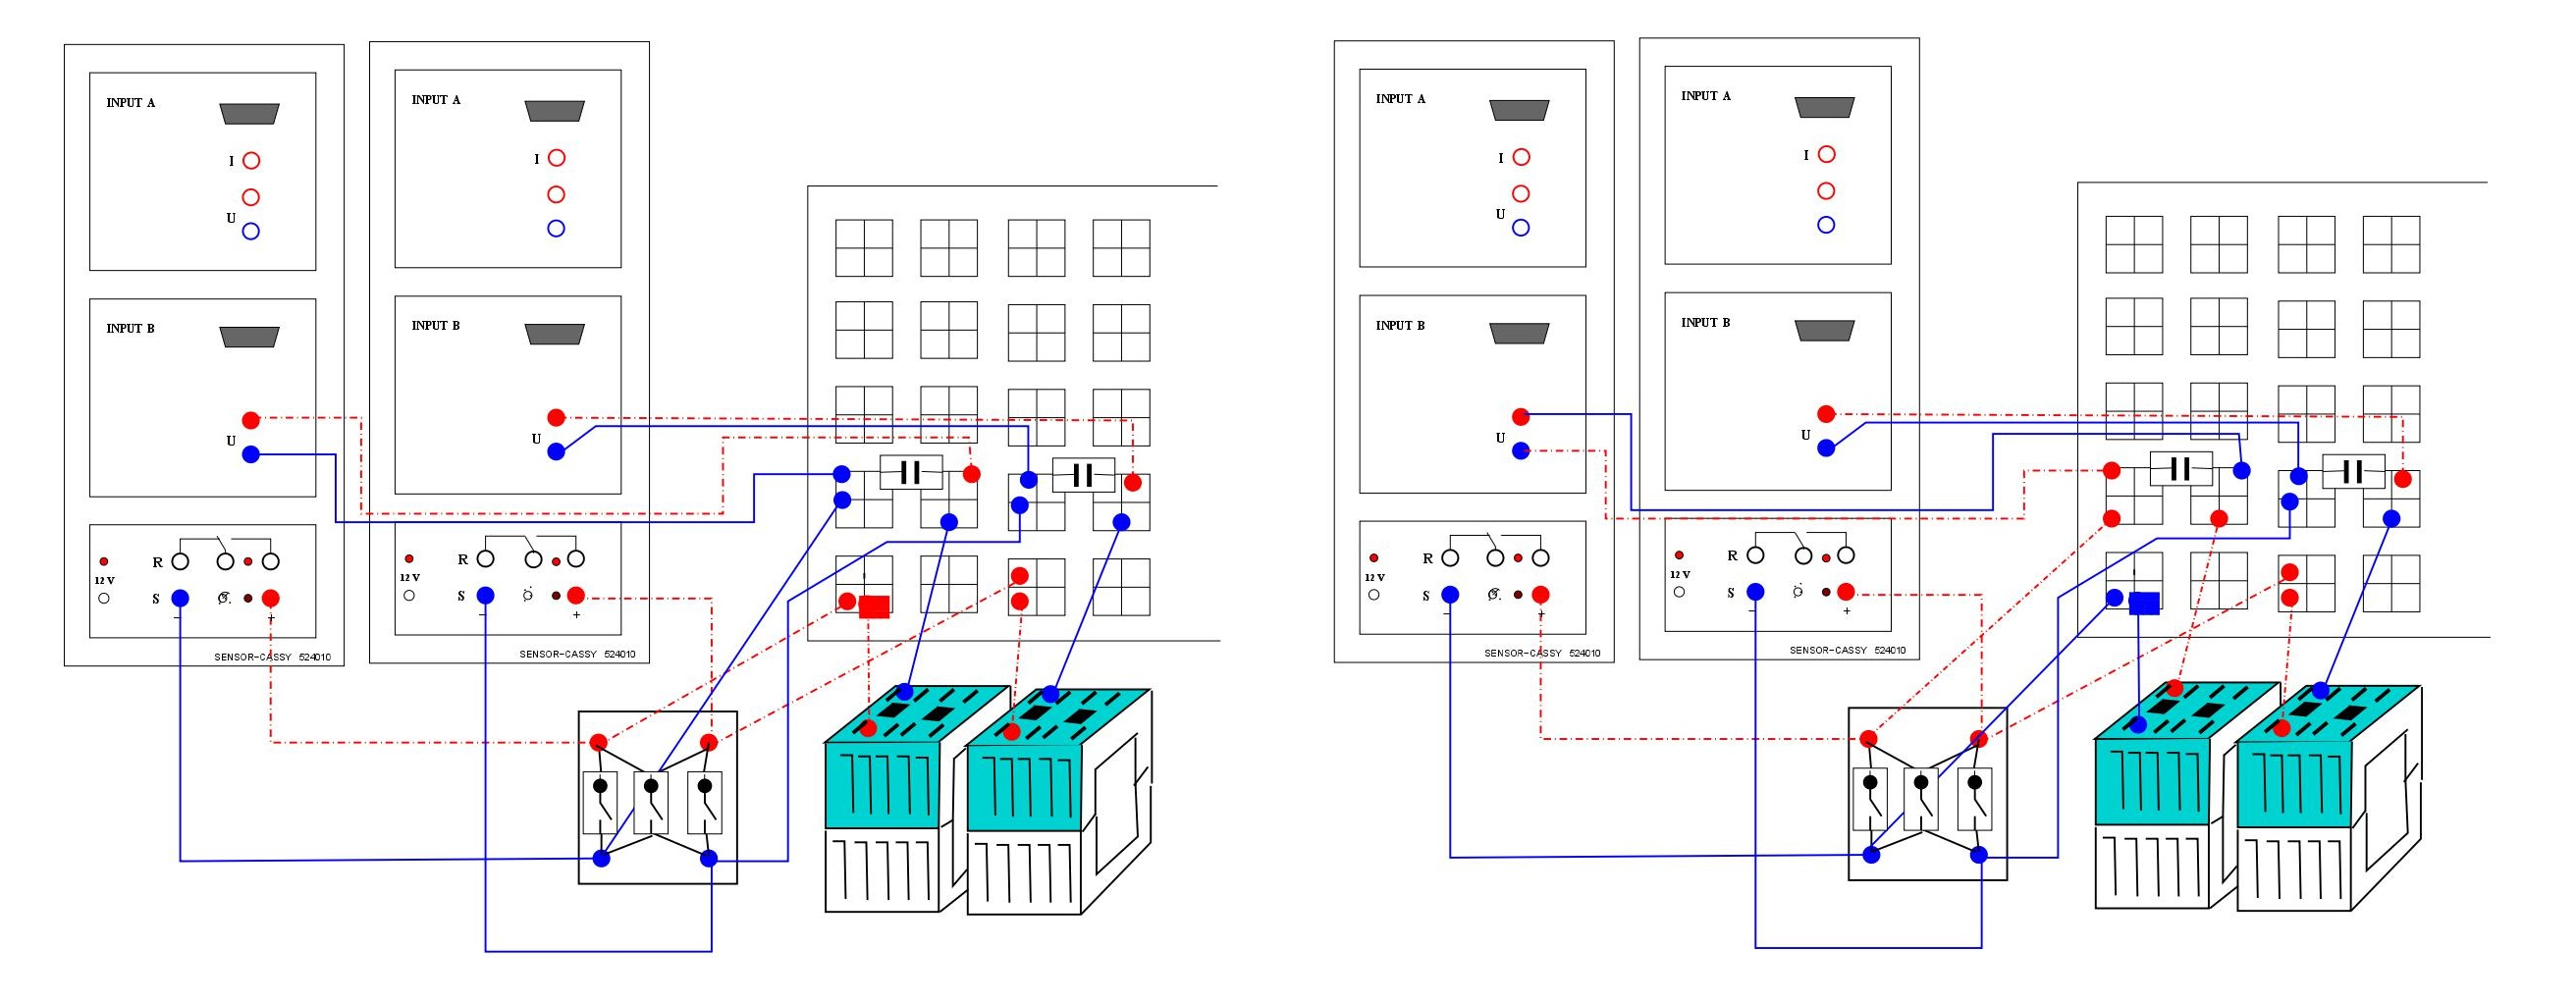
\includegraphics[width=\textwidth]{bilder/aufbau_fundamental.jpg}
\caption{Aufbau zur Anregung der Fundamentalschwingungen}
\label{abb:aufbau_fundamental}
\end{figure}

Zur Anregung der Fundamentalschwingungen werden die Aufbauten aus Abbildung \ref{abb:aufbau_fundamental} verwendet. Dabei ist links die gleichsinnige und rechts die gegensinnige Anregung zu sehen. Abweichend zur Zeichnung werden die Spannungen jeweils am Eingang A gemessen. Die Kondensatoren und Spulen sind dabei die gleichen wie bei der Aufzeichnung der Schwebung.

\subsubsection{Versuchsdurchführung}

Es werden die gleichen Messparameter wie bei der Aufzeichnung der Schwebung verwendet. Einzig die Anzahl an Messpunkten wird auf 16000 erhöht, entsprechend einer Messzeit von 160 ms. Dies dient der besseren Auflösung der Peaks im Frequenzspektrum. Die Messung wird wieder durch Betätigung des Schalters, welcher hier beide Schaltkreise gleichzeitig schaltet, gestartet. Die Spulen befinden sich ohne Eisenkern direkt aneinander.


\subsubsection{Versuchsauswertung}

Die Rohdaten zur gleichsinnigen Anregung sind in Abbildung \ref{abb:fundamental_roh} geplottet.  

\begin{figure}[H]
\centering
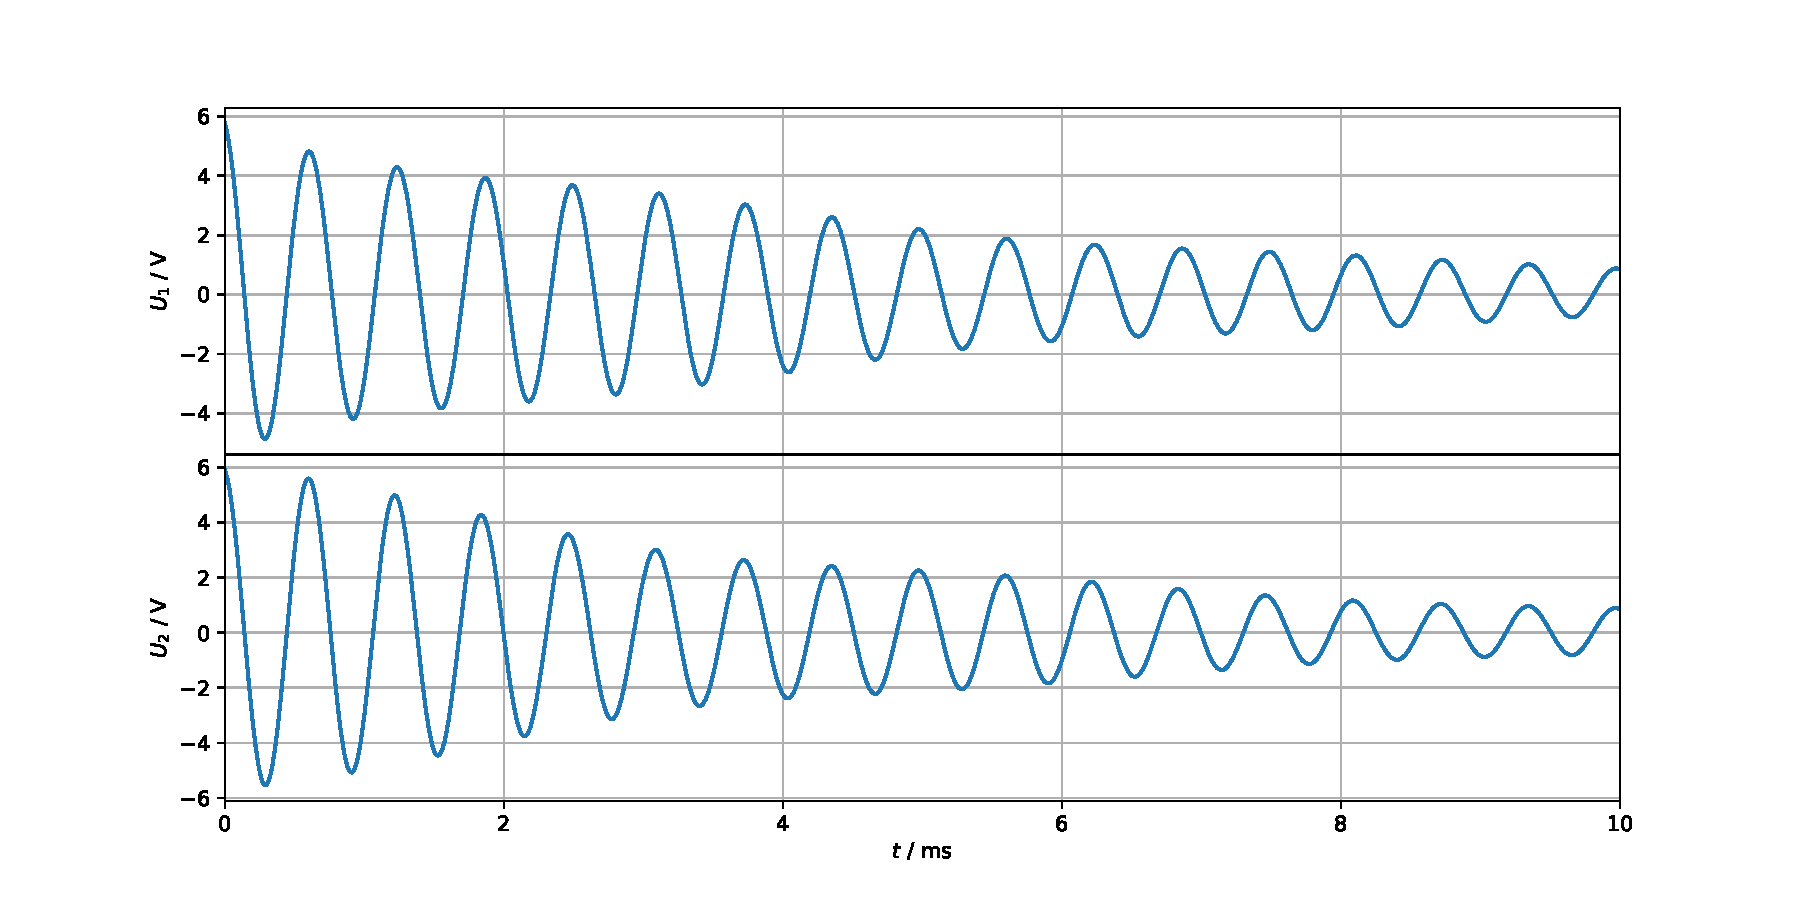
\includegraphics[width=\textwidth]{plots/fundamental_roh.pdf}
\caption{Rohdaten zur Anregung der gleichsinnigen Fundamentalschwingung}
\label{abb:fundamental_roh}
\end{figure}

Interessanter sind jedoch die Frequenzspektren der beiden Anregungen. Diese befinden sich in Abbildung \ref{abb:FFT_fundamental}.

\begin{figure}[H]
\centering
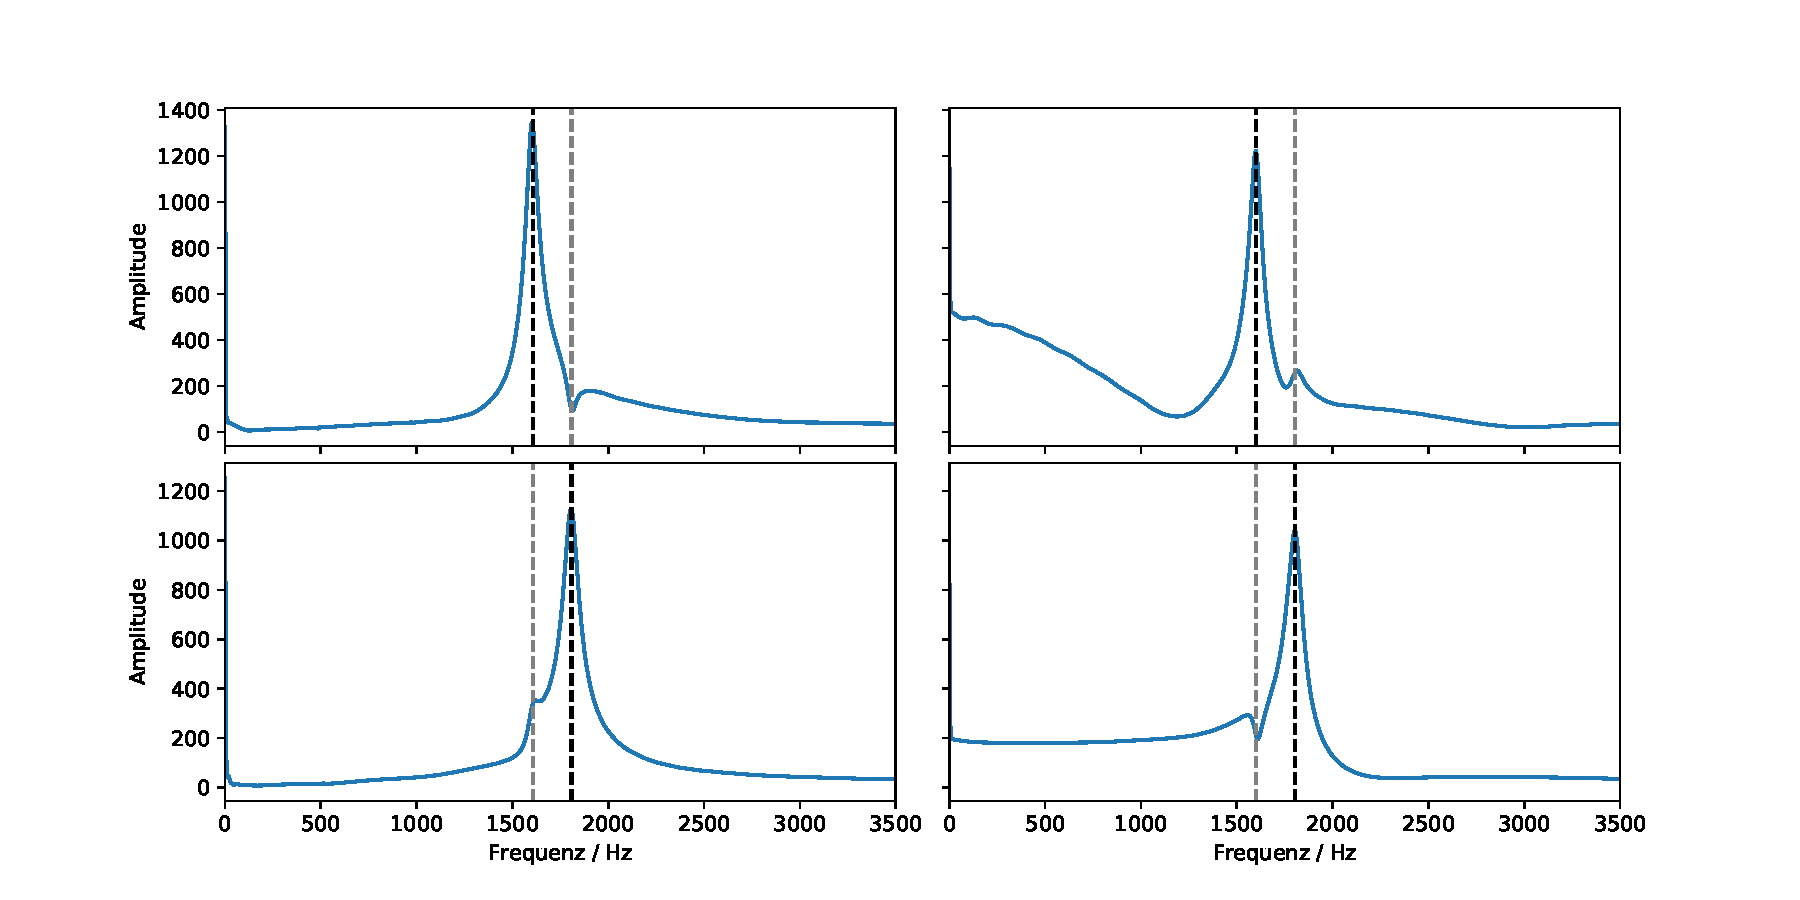
\includegraphics[width=\textwidth]{plots/fundamental_fft.pdf}
\caption{Frequenzspektren der Fundamentalschwingungen}
\label{abb:FFT_fundamental}
\end{figure}

Dabei sind oben die gleichsinnigen und unten die gegensinnigen Anregungen zu sehen. Zudem ist jeweils links der erste und rechts der zweite Schwingkreis. Die Frequenzen stimmen in etwa mit den Frequenzen aus Schwebung 1 überein. Die Abweichungen können vor allem durch der veränderten Aufbau bedingt sein.

\subsubsection{Fazit}

Es war äußerst schwierig die Fundamentalschwingungen zu treffen. Durch leicht unterschiedliche Bauteile und die schwierige gleichzeitige Schaltung der beiden Schwingkreise sind die erhaltenen Schwingungen eher Zufallsprodukte gewesen. Man sieht im Frequenzspektrum zudem, dass die zweite Fundamentalschwingung auch leicht angeregt wird.